\documentclass[a4paper]{article}

\usepackage{listings}
\lstset{language=bash, frame=single}
\usepackage{graphicx}
\usepackage[pdftex]{hyperref} % must go last!

\title{Remotely work with Jupyter(IPython) notebooks on the UCL Geography Linux cluster}
\author{Chad Stainbank}

\begin{document}
\maketitle
\section{Introduction}
\subsection{What is this?}

The \href{http://jupyter.org/}{Jupyter Notebook}~(previously IPython Notebook) provides a feature-rich interactive environment for learning and using \href{https://www.python.org/}{Python}.
If you're studying for a BSc or MSc at the University College London Department of Geography then it's likely that you've encountered these Notebooks in one or more of your modules or in the preparation of a dissertation.
Usually you will work with them from one of the collection of workstations in Pearson 110a that forms part of the \href{http://www.geog.ucl.ac.uk/resources/computer-support/teaching-cluster}{Geography Linux Cluster}.
Since physical access to Pearson 110a is not always practical, you may wish to have remote access to these files from another computer.
This guide will show you how to work with Jupyter Notebooks, hosted on the Linux Cluster, from your own computer. 

The bulk of this guide is written for somebody using the terminal on a Linux computer, the same OS running on the machines in Pearson 110A.
However, it is likely that your own computer runs on either \emph{Mac OS X} (\emph{macOS}) or \emph{Microsoft Windows}.
Since macOS is a \href{http://unix.stackexchange.com/questions/1489/is-mac-os-x-unix}{Unix-based} operating system, Apple fans should be able to enter all these same commands in Section \ref{sec:linuxmac} the \href{http://www.macworld.co.uk/feature/mac-software/get-more-out-of-os-x-terminal-3608274/}{Mac Terminal} with little modification.
For Windows users, on the other hand, there is a degree of set-up involved in order to get these commands to work: see Section \ref{sec:windows}.

\section{On Linux/ Mac OS X}
\label{sec:linuxmac}
\subsection{Manual}
\label{sec:manual}

The section provides a very explicit set of instructions to get up and running with remote Jupyter Notebooks.
The Listings boxes display commands to be entered into the terminal. \textbf{\textless{}\textgreater{}} enclose values which must be replaced as specified, while comments --- any text after \textbf{\#} --- do not need to be entered.
Since these commands may not always render properly, be careful to distinguish one dash ``-'' from two ``-{}-'' --- it should never be a long dash ``--''!
If you're familiar with the command-line interface then you could skip to Section \ref{sec:auto}, where they're condensed to shell functions, but it's probably worth going through this just once to make sure that everything is working smoothly.

\subsubsection{Run Notebook Server}
\label{sec:runnb}

The first step is use the program \href{http://linuxcommand.org/man_pages/ssh1.html}{SSH}~to remotely log into one of the machines in Pearson 110a and start up a Notebook server.
Because of the way the Linux cluster is set up, this requires a two-step (or ``multi-hop'') log in.
To make the first hop, open a new terminal and enter the command in Listing \ref{lst:logingw}, replacing \textless{}USER\textgreater{} with your UCL username and \textless{}GATEWAY\textgreater{} with the name of any one of the gateway servers listed on \href{http://www.geog.ucl.ac.uk/resources/computer-support/linux-remote-access}{Geography Remote Access page}.

\begin{lstlisting}[caption={Login to gateway}, label={lst:logingw}]
ssh <USER>@<GATEWAY>.geog.ucl.ac.uk
\end{lstlisting}

Enter your Geography network password \footnote{this is not necessarily the same password that you use for other UCL services.} when prompted, then enter the command in \ref{lst:loginws}.
Here, \textless{}MACHINE\textgreater{} must be replaced by the name of your favourite teaching workstation in Pearson 110a.

\begin{lstlisting}[caption={Login to workstation}, label={lst:loginws}]
ssh <MACHINE>
\end{lstlisting}

After entering your password again, start running the Notebook server with command \ref{lst:runnb}.
The flag ``--no-browser'' prevents Firefox from opening automatically, while ``--port'' tells the server to listen on a particular port number.
This is 8888 by default, although you can choose just about any integer above 1026 to replace \textless{}PORT\textgreater{}.

\begin{lstlisting}[caption={Run Notebook server}, label={lst:runnb}]
jupyter notebook --no-browser --port=<PORT>
\end{lstlisting}

Jupyter should now inform you that ``The IPython Notebook is running at: \textless{}link\textgreater{}''.
Without opening the link, check that the port number (after ``http://localhost:'') is the same the one you specified.
If it has changed, simply note down the new number and use it as \textless{}PORT\textgreater{} for all subsequent commands.

\subsubsection{Set up SSH tunnel}
\label{sec:tunnel}
The next step is to create create an \href{http://blog.trackets.com/2014/05/17/ssh-tunnel-local-and-remote-port-forwarding-explained-with-examples.html}{SSH tunnel}, through which you can connect to the Notebook server you just created.
In a \textbf{new} terminal, enter the commands in Listings \ref{lst:tunnel1} and \ref{lst:tunnel2}.
Here, the ``-L'' flags tell SSH to use \href{https://help.ubuntu.com/community/SSH/OpenSSH/PortForwarding}{local port forwarding} to transfer data between nodes. 
As before, replace the bracketed values and supply your password when prompted.

\begin{lstlisting}[caption={Tunnel to gateway server}, label={lst:tunnel1}]
ssh -L <PORT>:localhost:<PORT> -N <MACHINE>
\end{lstlisting}

\begin{lstlisting}[caption={Tunnel to machine}, label={lst:tunnel2}]
ssh -L <PORT>:localhost:<PORT> -N <MACHINE>
\end{lstlisting}

If all has gone well, the terminal will appear to be hanging \footnote{The optional ``-N'' flag prevents any more user input} and the SSH tunnel should be open.
To use the Notebook, copy the link produced in Section \ref{sec:runnb} (e.g.~\url{http://localhost:8888}) and paste it into the URL bar of your favourite browser. 
Congratulations, you should now be looking at the familiar Jupyter Notebook file browser. If not, see \ref{sec:trouble} 

\subsubsection{Troubleshooting}
\label{sec:trouble}
Occasionally, when trying to set up the SSH tunnel, you will get a message like:
\begin{quote}
bind: Address already in use

channel\emph{setup}fwd\_listener: cannot listen to port: \textless{}PORT\textgreater{}

Could not request local forwarding
\end{quote}

This means that the tunnel could not be established as another process is using that particular port.
If this occurs, start everything over again with a different port number.

\subsection{Automatic}
\label{sec:auto}

\subsubsection{Generate SSH keys}
\label{sec:sshkeys}
Following all the steps in \ref{sec:manual} require you to enter your password a total of four times, once for each SSH command.
\href{https://wiki.archlinux.org/index.php/SSH_keys}{\emph{SSH keys}} provide an alternative form of authentication, using a private and a public key to allow passwordless login over SSH.
Two seperate pairs of keys must be set-up: one for the initial hop from your computer to the gateway node, and the other for the onward hop to the workstation.

To set up the first pair of keys, open a terminal on your computer and enter the command:
\begin{lstlisting}[caption={Generate SSH keys}, label={lst:genkeys}]
ssh-keygen -t rsa
\end{lstlisting}
Let the program use the default file with no passphrase by presssing enter twice, then copy the public key to the geography file network using command \ref{lst:cpkeys} and following the instructions returned by the program.

\begin{lstlisting}[caption={Copy public key to geography file system}, label={lst:cpkeys}]
ssh-copy-id <USER>@<GATEWAY>.geog.ucl.ac.uk
\end{lstlisting}

To generate a pair of keys for the second hop, simply login to the any machine on the linux cluster and repeat the process.
\footnote{You do not need to specify \textless{}USER\textgreater{}, nor finish the address with ``.geog.ucl.ac.uk'', as you are already within the geography network.}

\subsection{Geography login/tunnel functions}
\label{sec:gfuncs}

It will very quickly become tedious to perfectly type out the commands in Section \ref{sec:manual} every time you want to run a Notebook remotely.
The two \href{https://www.shellscript.sh/functions.html}{functions}~in listing
\ref{lst:gfuncs} written for \href{http://cs.lmu.edu/~ray/notes/bash/}{bash}, condense all of these lines to a few short commands.

\lstinputlisting[float, floatplacement=hpb, caption={Functions to login/tunnel to geography cluster}, label={lst:gfuncs}, firstline=2, lastline=21, breaklines=true]{geog_functions.sh}

Be aware that Listing \ref{lst:gfuncs} is for demonstration only; it does not display properly in a pdf document and so will not work if used as-is.
Instead, raw text file containing these functions can be found at:

\noindent\small\url{https://github.com/stainbank/remote_ipynb/blob/master/geog_functions.sh}

The simplest way to ``install'' these two functions is to paste the entire code block --- replacing the defaults as appropriate --- into a file in your home directory called \href{http://superuser.com/questions/49289/what-is-the-bashrc-file}{.bashrc}~file.
If this file doesn't already exist, \href{http://apple.stackexchange.com/a/119714}{as is the case on Mac OS X}, simply create it and then add the following line to the file .bash\_profile~(also in the user root directory):

\begin{lstlisting}[caption={Source .bashrc on startup}, label={lst:srcbashrc}]
if [ -f ~/.bashrc ]; then . ~/.bashrc; fi
\end{lstlisting}

The command \emph{geog} replaces the commands in Listings \ref{lst:logingw} and \ref{lst:loginws}, while \emph{geogport} replaces \ref{lst:tunnel1} and \ref{lst:tunnel2}.
You can therefore work with a remote notebook by simply entering:
\begin{lstlisting}[caption={Set up and tunnel to remote Notebook server}, label={lst:usegfuncs}]
# In one terminal
geog
jupyter notebook --no-browser --port=<PORT>
# In another terminal
geogport
\end{lstlisting}

These functions also take positional arguments, in the order:

\emph{geog} \textless{}MACHINE\textgreater{} \textless{}GATEWAY\textgreater{} \textless{}USER\textgreater{}
\emph{geogport} \textless{}PORT\textgreater{} \textless{}MACHINE\textgreater{} \textless{}GATEWAY\textgreater{} \textless{}USER\textgreater{}

This allows you to change any variables from their default values \footnote{You must supply all \emph{preceeding} arguments; prefix the an argument name with \textbf{\$} to use the default value}:

\begin{lstlisting}[caption={Examples of arguments to geography login/tunnel functions}, label={lst:gfuncsargseg}]
geog ulanbator # change machine
geog $MACHINE triangle ucfaxyz # change user and gateway
geogport 8889 # change port
geogport $GPORT lima # change machine
\end{lstlisting}

\section{On Windows}
\label{sec:windows}

Sections \ref{sec:wsl} and \ref{sec:putty} describe how to setup a Windows terminal emulator, into which you can enter commands adapted from Section \ref{sec:linuxmac}.
Since much of the material here refers to that section, you must read it first.
However, I strongly urge any Windows users intending on working extensively with Python and Jupyter Notebooks to consider installing a Linux distribution\ldots

\subsection{Install Linux}
\label{sec:win2lnx}
Don't be alarmed: this need not be a drastic switch as there are two simple ways to set up Linux \emph{alongside} Windows.
The first is to use a \emph{\href{https://www.howtogeek.com/196060/beginner-geek-how-to-create-and-use-virtual-machines/}{virtual machine}}, an OS that runs \emph{inside} your current system.
This is very simple to setup (see \href{http://www.storagecraft.com/blog/the-dead-simple-guide-to-installing-a-linux-virtual-machine-on-windows/}{here}) and I myself use this method to work from UCL's library computers.

The second option, and the one I use for my personal computer, is \emph{\href{https://www.howtogeek.com/187789/dual-booting-explained-how-you-can-have-multiple-operating-systems-on-your-computer/}{dual-booting}}.
Although this imay seem somewhat involved, a native Linux install is always faster than a virtual one and there are plenty of guides available online to guide you through the process (e.g.\href{https://itsfoss.com/guide-install-linux-mint-16-dual-boot-windows/}{1}, \href{https://www.lifewire.com/ultimate-windows-7-ubuntu-linux-dual-boot-guide-2200.53}{2}, \href{https://www.howtogeek.com/214571/how-to-dual-boot-linux-on-your-pc/}{3}, \href{http://www.pcworld.com/article/2955460/operating-systems/dual-booting-linux-with-windows-what-you-need-to-know.html}{4}). 

Whichever installation option you go for, you will need to choose one from among the many \emph{\href{http://distrowatch.com/dwres.php?resource=major}{distributions}} of Linux, with \href{https://www.ubuntu.com/download}{Ubuntu}~and \href{https://linuxmint.com/}{Linux Mint} most often suggested for beginners. For use on a virtual machine or an ageing laptop, I would recommend opting for a more lightweight flavour --- i.e. on that features MATE, Xfce or LXDE as it's desktop environment.

\subsection{Windows Subsystem for Linux}
\label{sec:wsl}
If you have Windows 10 then you'll be able to take advantage of a new Microsoft development called \emph{Windows Subsystem for Linux} (WSL), otherwise referred to as \emph{Bash on Ubuntu on Linux}, which provides a Linux command-line interface on Windows.
To use WSL to run Jupyter Notebooks, simply \href{https://msdn.microsoft.com/en-gb/commandline/wsl/install_guide}{install the feature} then follow the instructions above for Linux.

\subsection{PuTTY}
\label{sec:putty}

If you don't have access to WSL then you'll have to use the popular terminal emulator and SSH client \emph{PuTTY} to access your Notebooks. 
First install the program from its \href{http://www.chiark.greenend.org.uk/~sgtatham/putty/latest.html}{website}, then run a PuTTY instance to load its GUI configuration screen. 
Navigate to the \emph{Session} screen and enter \textless{}USER\textgreater{}@\textless{}GATEWAY\textgreater{}.geog.ucl.ac.uk in the \emph{Host Name} box, making the appropriate replacements (described in Section \ref{sec:linuxmac}).
\footnote{Follow \href{http://www.geo.mtu.edu/geoschem/docs/putty_install.html}{this guide} if you want to be able to load X11 windows (i.e. graphical programs such as~\emph{gedit}~or~\emph{Firefox}), although this is not necessary for using Notebooks.}
To store these gateway login settings, enter a name under \emph{Saved Sessions} and click \emph{Save} (Figure \ref{fig:putty1}).
To set up the SSH tunnel, ensure that the settings from the previous session are loaded, then navigate to the port forwarding options via \emph{Connection} \textgreater{} \emph{SSH} \textgreater{} \emph{Auth} \textgreater{} \emph{Tunnels} (Figure \ref{fig:putty2}). 
Under \emph{Source Port} supply \textless{}PORT\textgreater{} and enter 127.0.0.1:\textless{}PORT\textgreater{} as the \emph{Destination}, substituting \textless{}PORT\textgreater{} with a valid port number as described in Section \ref{sec:runnb}.
Click the \emph{Add} button to commit this information to the list of \emph{Forwarded ports}.
Finally, to save these settings, navigate back to \emph{Sessions} and enter a \textbf{new} name under \emph{Saved Sessions} before clicking \emph{Save} (Figure \ref{fig:putty3}).

\begin{figure}[p]
  \centering
    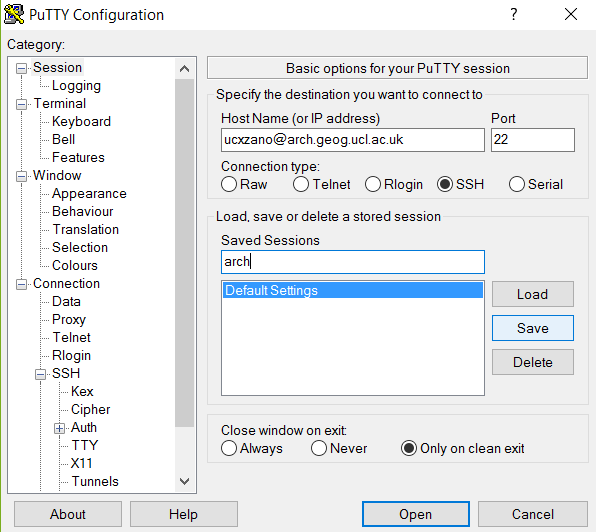
\includegraphics[width=\textwidth]{figures/putty1_save_login_session.png}
  \caption{Save session to login to gateway}
  \label{fig:putty1}
\end{figure}

\begin{figure}[p]
  \centering
    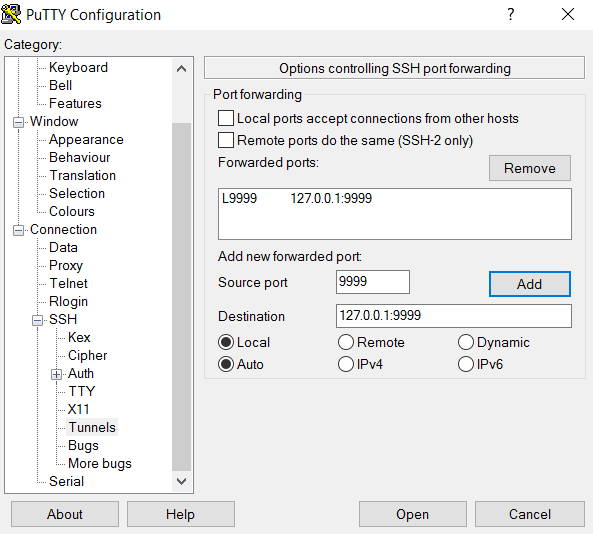
\includegraphics[width=\textwidth]{figures/putty2_setup_tunnel.png}
  \caption{Set up port forwarding to gateway}
  \label{fig:putty2}
\end{figure}

\begin{figure}[p]
  \centering
    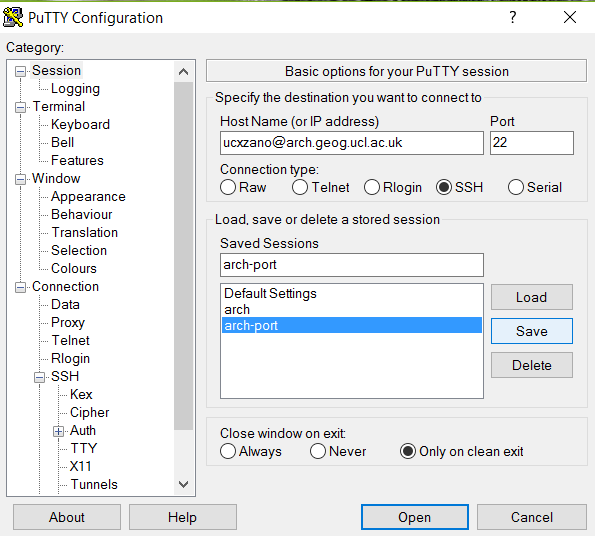
\includegraphics[width=\textwidth]{figures/putty3_save_tunnel_session.png}
  \caption{Save session to tunnel to gateway}
  \label{fig:putty3}
\end{figure}
\end{document}

To work with Jupyter Notebook on the Geography Linux Cluster, open each of these session profiles in individual PuTTY windows.
The first session you created (\emph{arch} in Figure \ref{fig:putty1}) replaces the command in Listing \ref{lst:logingw}, while the second (\emph{archport} in \ref{fig:putty3}) replaces Listing \ref{lst:tunnel1}. Therefore, to remotely work with a Jupyter Notebook, simply substitute these while following the instructions in Section \ref{sec:manual}.

\end{document}
